\documentclass[a4paper,12pt]{article}

% Author and title
\def\MYDIRECTOR{Մարիամ Հարությունյան}
\def\MYDIRECTORTITLE{ֆիզ.-մաթ. գիտ. դոկտոր, պրոֆեսոր}
\def\MYAUTHOR{Բաբկեն Վարդանյան}
\author{\MYAUTHOR}
\def\MYTITLE{Սերվերային համակարգերի անվտանգությունը գնահատող ծրագրի մշակում}
\title{\MYTITLE}
\date{2016}

% Packages
\usepackage{polyglossia}
\usepackage[hyphens]{url}
\usepackage{listings}
\usepackage{graphicx}
\usepackage{color}
\usepackage{hyperref}
\usepackage{fancyhdr}
\usepackage[titles]{tocloft}
\usepackage{pdfpages}
\usepackage{indentfirst}
\usepackage[top=20mm, bottom=20mm, left=30mm, right=10mm]{geometry}
\usepackage{setspace}
\usepackage{tabularx}
\usepackage{titlesec}

% Fonts
\newfontfamily{\armenianfont}{GHEA Grapalat}
\newfontfamily{\armenianfonttt}{DejaVu Sans Mono}
\newfontfamily{\armenianmathfont}{GHEA Grapalat}
\ExplSyntaxOn
\DeclareSymbolFont{armenianletters}{\g_fontspec_encoding_tl}{\l_fontspec_family_tl}{m}{it}
\int_step_inline:nnnn { "531 } { 1 } { "556 }
{
\Umathcode #1 = "0 \symarmenianletters #1 % low level call
}
\int_step_inline:nnnn { "561 } { 1 } { "587 }
{
\Umathcode #1 = "0 \symarmenianletters #1
}
\ExplSyntaxOff

% Language
\setmainlanguage{armenian}

% Setup colors
\definecolor{bluekeywords}{rgb}{0,0,1}
\definecolor{greencomments}{rgb}{0,0.5,0}
\definecolor{redstrings}{rgb}{0.64,0.08,0.08}
\definecolor{xmlcomments}{rgb}{0.5,0.5,0.5}
\definecolor{types}{rgb}{0.17,0.57,0.68}

% Setup lst
\lstset{
  language={},
  showtabs=false,
  tabsize=4,
  breaklines=true,
  breakatwhitespace=false,
  breakindent=2.42em,
  showstringspaces=false,
  escapeinside={(*@}{@*)},
  commentstyle=\color{greencomments},
  keywordstyle=\color{bluekeywords},
  stringstyle=\color{redstrings},
  basicstyle=\armenianfonttt\footnotesize,
  caption=\getlstname
}
\makeatletter
\def\lst@lettertrue{\let\lst@ifletter\iffalse}
\makeatother
\makeatletter
\DeclareRobustCommand{\getlstname}{%
 \begingroup
  % \lstname seems to change hyphens into \textendash
  \def\textendash{-}%
  \filename@parse{\lstname}%
  \texttt{\filename@base.\filename@ext}%
 \endgroup
}
\makeatother

% Setup hyper
\hypersetup{
    colorlinks=false, %set true if you want colored links
    linktoc=all,     %set to all if you want both sections and subsections linked
}

% Setup linespread
\linespread{1.25}

% Setup URL
\urlstyle{tt}

% Renames
\renewcommand*\contentsname{Բովանդակություն}
\renewcommand{\figurename}{Նկար}
\renewcommand{\lstlistingname}{Սկզբնական կոդ}
% Start new page after section
\newcommand{\sectionbreak}{\clearpage}


%%%%%%%%%%%%%%%%%%%%%%%%%%%%%%%%%%%%%%%%%%%%%%%%%%%%%%%%%%%%%%%%%%%%%%%%%%%%%%%
\begin{document}

% Title page
\begin{titlepage}
	\centering
	{\LARGE
		\textit{ՀՀ ԿՐԹՈՒԹՅԱՆ ԵՎ ԳԻՏՈՒԹՅԱՆ ՆԱԽԱՐԱՐՈՒԹՅՈՒՆ} \par
		\textit{ՀՀ ԳԱԱ ԳԻՏԱԿՐԹԱԿԱՆ ՄԻՋԱԶԳԱՅԻՆ ԿԵՆՏՐՈՆ} \par
		\textit{ՄԱԳԻՍՏՐՈՍԱԿԱՆ ԹԵԶ} \par
		\textit{Բաբկեն Վարդանյան Սամվելի} \par
	}

	\vspace{2.5cm}

	\raggedright
	{\Large
		\begin{tabularx}{\textwidth}{ p{6.5cm} X }
		Մասնագիտություն` & Ինֆորմատիկա և հաշվողական տեխնիկա \\
		Թեմա՝ & \MYTITLE \\
		Գիտական ղեկավար՝ & \MYDIRECTORTITLE \ \MYDIRECTOR \\
		\end{tabularx}
	}

	\vspace{2cm}

	{\Large Թույլատրել պաշտպանության '$\rule{1cm}{0.15mm}$' '$\rule{3cm}{0.15mm}$' 2016 թ. \par}

	\vspace{2cm}
	{\Large
	}
	{\Large
		\begin{tabularx}{\textwidth}{ p{6.5cm} X }
		Ամբիոնի վարիչ` & Ֆիզ.-մաթ. գիտ. թեկնածու, դոցենտ Վլադիմիր Սահակյան \\
		\end{tabularx}
	}

	\centering
	\vfill
	{\Large ԵՐԵՎԱՆ 2016\par}
\end{titlepage}
\newpage

% Setup page numbering
\pagenumbering{arabic}
\setcounter{page}{2}

% Rest of the document
Կցանկանայի խորին երախտագիտությունս հայտնել իմ ղեկավար, \MYDIRECTORTITLE \
\MYDIRECTOR ին (ԻԱՊԻ), ով ինձ աջակցել և խրախուսել է այս աշխատանքի
ժամանակ:

\hfill \hfill Բաբկեն Վարդանյան

\newpage

\tableofcontents

\begin{sloppypar}
\section{Առաջաբան}


\subsection{Ի՞նչ է տեղեկատվական անվտանգությունը}

Տեղեկատվական անվտանգությունը տեղեկատվական ռեսուրսների չլիազորված օգտագործման
կանխման և հայտնաբերման պրոցեսն է [23]:

Տեղեկատվական ռեսուրսների չլիազորված օգտագործման
կանխումը չարամիտ չլիազորված անձանց (նաև ասում են «հակառակորդներ»,
«հարձակվողներ», «ներխուժողներ», «հաքերներ») կողմից ծրագրային ապահովման կամ
տվյալների որոշ մասի օգտագործման դեմ ուղղված միջոցառումների համակարգն է:

Տեղեկատվական ռեսուրսների չլիազորված օգտագործման
հայտնաբերումը չլիազորված մուտքի փորձի առկայության ստուգման պրոցեսն է: Եթե
նման փորձ առկա է, ապա նաև՝ արդոք այն հաջողվել է, և թե կոնկրետ ինչ է տեղի
ունեցել [20]:

\subsection{Ինչու՞ հոգալ տեղեկատվական անվտանգության մասին}

Այսօր համակարգիչները և էլեկտրոնային տեխնիկան օգտագործվում են
կյանքի գրեթե բոլոր ոլորտներում: Բանկային համակարգի ու ներդրումների ոլորտից
մինչև գնումների և հեռահաղորդակցության ոլորտ համակարգիչները դարձել են
յուրաքանչյուր բիզնեսի անբաժանելի մասը: Դժվար է նշել մի ոլորտ, որը
օգուտ չի քաղել տեղեկատվական տեխնոլոգիաների բուռն զարգացումից:

Չնայած ընկերությունների կողմից պահվող ոչ բոլոր տվյալները կարելի է
դասակարգել որպես «հույժ գաղտնի», ցանցային ադմինիստրատորները հավանաբար
չեն ուզենա որ անծանոթ անձինք հնարավորություն ունենան հետևել
իրենց ընկերության ներքին հաղորդակցությանը,
իրենց անձնական ինֆորմացիային, կամ փոփոխություններ կատարեն իրենց վստահված
համակարգերում:

Այդ պատճառով տեղեկատվական անվտանգությունը մնում է բիզնեսի և հասարակության
առջև ծառացած ամենակարևոր չհաղթահարված խնդիրներից մեկը [21]:

Սերվերի ղեկավարման հնարավորությունը հակառակորդի կողմից ռիսկի տակ է
դնում ոչ միայն ընկերությանը, այլ նաև ընկերության հաճախորդներին, ինչպես օրինակ
օրինակ վեբ կայքի այցելուներին:


\subsection{Ինչու՞ ինչ-որ մեկը կցանկանա կոտրել որոշակի համակարգ}


Հակառակորդներին հաճախ չի հուզում, թե ով է օգտագործողը կամ ընկերությունը,
որի վրա իրականացվում է հարձակումը:

Հակառակորդի հիմնական նպատակներն են՝

\begin{itemize}
\item \textbf{Դրամական եկամուտ} \\
	Կոտրված համակարգչից կամ սերվերից օգտագործողի
    կամ ընկերության բանկային հաշվի և վարկային քարտի տեղեկությունները
    գողանալու միջոցով:
\item \textbf{Բիզնեսի աշխատանքի խոչնդոտում} \\
	Մի ընկերություն կարող է վարձել
    հակառակորդին իրենց մրցակցի համակարգչային ցանցում քաոս ստեղծելու
    նպատակով:
\item \textbf{Ինֆորմացիայի գողություն} \\
	Մի ընկերություն կարող է վարձել
    հակառակորդին իրենց մրցակից ընկերության գաղտնիքները գողանալու և
    այդպիսով մրցակցային առավելություն ձեռք բերելու նպատակով:
\item \textbf{DDoS (Distributed Denial of Service - Բաշխված Ծառայության Ընդհատման գրոհ) գրոհներ
    իրականացնելու նպատակով այլ սերվերների վրա} \\
	DDoS գրոհի նպատակն է սերվիսը անհասանելի դարձնել`
	դրան տարբեր աղբյուրներից չափազանց շատ հարցումներ
	իրականացնելու միջոցով [32]:
	
    Նման հարձակման դեպքում կոտրված սերվերների քանակը
	ուղիղ համեմատական է գրոհի հաջողությանը:
\item \textbf{SEO (Search Engine Optimization - Որոնման համակարգերի օպտիմալացում)} \\
	Կոտրված կայքը կարող է
    օգտագործվել այլ կայքերի SEO-ն բարձրացնելու նպատակով՝ կոտրված կայքում
    տեղադրելով հղումեր դեպի այդ կայքը:
\item \textbf{Հենակետ հետագա գրոհների համար} \\
	Կոտրված սերվերը կարող է օգտագործվել
	որպես հենակետ`
	\begin{itemize}
	\item նույն ընկերության ցանցում հետագա ավելի լայնածավալ հարձակումների
		համար,
	\item ավելի շատ սերվերներին տիրանալը օգնում է հակառակորդին թաքցնել
		իր ինքնությունը (IP հասցեն)՝ այլ ընկերությունների դեմ հետագա
		հարձակումների ժամանակ:
	\end{itemize}
\item \textbf{Զվարճանք} \\
	Հակառակորդը կարող է կոտրել սերվերը զուտ հետաքրքրության կամ
    զվարճանքի համար:
\end{itemize}


\subsection{Սերվերային անվտանգության ժամանակակից պրակտիկան}


Սերվերների անվտանգությունը ապահովելու այսօր ընդունված ամենատարածված
պրակտիկաներից են [21]՝

\begin{enumerate}
\item \textbf{Անջատել կամ ջնջել ոչ անհրաժեշտ սերվիսները}\\
    Օպերացիոն համակարգերի լռելյայն կոնֆիգուրացիան երբեմն ապահով չէ:
    Սովորաբար տեղադրված են բազմաթիվ չօտագործվող սերվիսներ, ինչպես
    օրինակ՝ պրինտ սերվերը, «Սամբա» ֆայլերի բաշխման համակարգը և այլն:
	Այս սերվիսները
    մեծացնում են հարձակման հարթությունը, բացելով ավելի շատ հնարավոր եղանակներ
    չարամիտ օգտագործողի համար՝ համակարգը չարաշահելու նպատակով:

    Ադմինիստրատորները պետք է անջատեն կամ մեկուսացնեն բոլոր չօգտագործվող
    սերվիսները, օրինակ՝ firewall-ի օգնությամբ:
\item \textbf{Հեռակառավարում}\\
    Չպաշտպանված, հանրային ցանցերով մուտքը սերվեր հնարավոր է դարձնում
    հակառակորդների կողմից տարաբնույթ հարձակումներ, ինչպիսին է
    մարդը մեջտեղում (man-in-the-middle) և տվյալների գողություն:

    Ադմինիստրատրոը պետք է համոզվի, որ բոլոր հեռակառավարման կապերը
    դեպի սերվեր պաշտպանված են գաղտնագրմամբ և գաղտնաբառով:
\item \textbf{Թույլտվություններ և արտոնություններ}\\
    Թույլտվությունների հստակ կառավարման համակարգը կարևոր դեր է խաղում
    սերվերային անվտանգության մեջ: Եթե չարամիտ օգտագործողը կամ պրոցեսը
    ունենա ավելի շատ արտոնություններ, քան իրեն անհրաժեշտ է, այդ հանգամանքը
    կարող է նպաստել սերվերի կոտրմանը:

    Ադմինիստրատորը պետք է համոզվի, որ բոլոր օգտագործողները մուտք ունեն
    միայն այն ֆայլերին և ռեսուրսներին, որոնք իրենց անհրաժեշտ են
    աշխատանքը իրականացնելու համար, և ոչ ավելին:
\item \textbf{Ժամանակին տեղադրել անվտանգության թարմացումները}\\
    Կարևոր է տեղադրել օպերացիոն համակարգը և ծրագրային ապահովումը
    վերջին թարմացումներով և անվտանգության կարկատաններով (patches):

	Օպերացիոն համակարգի և ծրագրային ապահովման ստեղծողները ժամանակ
	առ ժամանակ թողարկում են թամացումներ (updates):
	Դրանք հաճախ պարունակում են անվտանգության թարմացումներ, որոնք
	փակում են հայտնաբերված խոցելիություններն օպերացիոն համակարգում:

    Ադմինիստրատորները պետք է համոզվեն որ թարմացումները տեղադրվում են
    ժամանակին:
\item \textbf{Դիտարկում և գրանցամատյանների գրառումների (logs) հաշվեքննություն}\\
    Լոգեր ստեղծվում են բոլոր տեսակի ծրագրային ապահովման կողմից -
    օպերացիոն համակարգի, վեբ հավելվածների, բոլոր տեսակի սերվիսների,
    տվյալների բազաների, ցանցային սարքերի, երթուղավորիչների, կոմուտատորների (network switch)
	և այլն կողմից:

    Այս լոգերը պետք է դիտարկվեն և հաճախ ստուգվեն, քանի որ դրանք երբեմն
    կարող են զգուշացնել վերահաս վտանգի մասին: Նույնիսկ հաջող հարձակման
    դեպքում սերվերների լոգերը հաճախ դատական փորձաքննություն
    իրականացնելու միակ միջոցն են:
\item \textbf{Օգտագործողի հաշիվներ}\\
    Չօգտագործվող օգտագործողի հաշիվները, ինչպիսիք են աշխատանքից ազատված
    աշխատակիցների հաշիվները, պետք է անջատվեն: Պետք է անջատվեն նաև զանազան
    չօգտագործվող սերվիսների կողմից ստեղծված օգտագործողների հաշիվները:

	Յուրաքանչյուր օգտագործողի հաշիվ մեծացնում է հարձակման հարթությունը:
	Նախկին աշխատակիցը կարող է ընկերությանը վնաս հասցնելու դրդապատճառներ
	ունենալ, և եթե նրա օգտագործողի հաշիվը անջատված չլինի՝
	նա հնարավորություն կունենա ցանկացած գործողություն կատարել
	իր օգտագործողի իրավասություններով:

    Յուրաքանչյուր ադմինիստրատոր և օգտագործող, ով մուտք է գործում
    սերվեր, պետք է ունենա իր սեփական հաշիվը և գաղտնաբառը, և ճիշտ
    իրավասություններ: Գաղտնաբառը չպետք է բաշխվի օգտագործողնեիր միջև:
\item \textbf{Ջնջել չօգտագործվող մոդուլներ և ընդլայնումներ}\\
    Հավելվածները, ինչպես օրինակ վեբ սերվերները, հաճախ կարող են պարունակել
    որոշակի լռելյայն ընդլայնումներ և ծրագրային միավորներ (modules):
    Այս ծրագրային միավորները կարող են պարունակել խոցելիություններ, և
    այդպիսով մեծացնել հնարավոր հարձակման հարթությունը հակառակորդի համար:

    Ադմինիստրատորը պետք է համոզվի, որ հնարավորության դեպքում միայն
    վեբ հավելվածների համար անհրաժեշտ միավորներն են առկա:
\item \textbf{Լինել տեղեկացված}\\
    Այսօր օպերացիոն համակարգերի և ծրագրային ապահովման,
    այդ թվում՝ դրանց անվտանգության մասին ինֆորմացիան ազատորեն հասանելի է
    համացանցում:

    Ադմինիստրատորները պետք է համոզվեն, որ իրենք և իրենց օգտագործողները
    մշտապես տեղեկացված են հարձակումների և խոցելիությունների մասին
    վերջին նորություններին:
\item \textbf{Օգտագործել սկզբնական կոդի (source code) անվտանգության սկաներներ}\\
    Սկաներները ծրագրեր են, որոնք ավտոմատացնում և հեշտացնում են սերվերի
    և հավելվածների պաշտպանության գործընթացը:

    Ծրագրային կոդի ստատիկ և դինամիկ անալիզի գործիքները, ինչպիսիք են
    Sonar -ը Java լեզվի համար, Valgrind-ը C լեզվի համար և այլն,
    օգնում են գտնել ծրագրային սխալներ (bugs) և խոցելիություններ ծրագրի
    կենսափուլի (lifecycle) վաղ շրջանում:
\item \textbf{Ընտրել գաղտնագրման և հեշավորման ապահով ալգորիթմներ}\\
    Պետք է խուսափել կոտրված գաղտնագրման, հաղորդակցության և
    հեշավորման հաղորդակարգերի օգտագործումից, ինչպիսիք են՝
	DES, SSL, MD5:

    Այս հաղորդակարգերի թուլությունը հարձակման հնարավոր
    վեկտոր է բացում հակառակորդի համար:

    Այսպիսի հաղորդակարգերը պետք է փոխարինվեն ժամանակակից,
    չկոտրված և գաղտնագրման լայն հանրության վստահությանը արժանացած
    հաղորդակարգերով:
\item \textbf{Օգտագործել հակավիրուս}\\
	Windows օպերացիոն համակարգի վրա հիմնված սերվերներում անհրաժեշտ է տեղադրել
	հակավիրուսային ծրագրային ապահովում [16]:

	Հակավիրուսը սկանավորում է ծրագիրը հետևյալ պայմաններում՝
	\begin{enumerate}
		\item ամբողջական սկաներ - թողարկվում են պարբերաբար կամ օգտագործողի կողմից,
		\item աշխատանքի ժամանակ, այսինքն երբ համակարգով փոխանցվում են տվյալներ:
	\end{enumerate}

	Հակավիրուսները օգտագործում են վիրուսների հայտնաբերման հետևյալ տեխնոլոգիաները՝

	\begin{enumerate}
	\item ստորագրության վրա հիմնված հայտնաբերում, երբ ֆայլը համեմատվում է հայտնի չարամիտ կոդի հետ,
	\item փորձարարության վրա հիմնված հայտնաբերում, երբ ֆայլի վարվելաձևը համեմատվում է հայտնի չարամիտ նմուշների հետ,
	\item վարվելակերպի վրա հիմնված հայտնաբերում, որը հաճախ կատարվում է ՆՀՀ-երում:
	\end{enumerate}

	Linux-ի վրա հիմնված համակարգերում հակավիրուս հաճախ չի օգտագործվում [17]:

	Linux-ի վրա հիմնված համակարգերում հակավիրուսի անհրաժեշտություն կարող է
	առաջանալ միայն այն պարագայում, երբ այն օգտագործվում է Windows համակարգերի
	միջև ֆայլերի փոխանակաման համար [19]:
\item \textbf{Օգտագործել ցանցային սկաներներ}\\
    Ցանցային սկաներները օգնում են ադմինիստրատորներին համոզվել իրենց
    սերվերների անվտանգության մեջ: Այսպիսի գործիքները կարողանում են
    հայտնաբերել բաց պորտեր, խոցելի սերվիսներ, և նույնիսկ վիրուսներ:
    Հայտնի ցանցային սկաներնեից են՝
    \begin{enumerate}
        \item Nmap,
        \item Nessus,
        \item Acunetix:
    \end{enumerate}
	Համակարգային ադմինիստրատորների տարածված պարտականություններից է իրենց
	վստահված համակարգերում պորտերի սկանավորման իրականացումը:
	Այսպիսի սկանավորումները օգնում են ադմինիստրատորներին գտնել խոցելիություններ
	իրենց համակարգերում ավելի վաղ, քան հնարավոր հակառակորդը:
	Ցանցային պորտերի սկանավորման պրոցեսը հաճախ ունի ներքոնշյալ հաջորդականությունը:

	\begin{enumerate}
	\item Ադմինիստրատորը որոշում է հասցեների և պորտերի շրջանակը, որոնք պետք է
		ենթարկվեն սկանավորման:
	\item Նա ցանցային սկաներին է տալիս այդ պարամետրերը և սկսում է
		սկանավորման գործընթացը:
	\item Ծրագիրը փորձարկում է IP հասցեների և պորտերի բոլոր տրված
		համադրությունները:
	\item Եթե պարզվում է, որ պորտը բաց է, ապա աշխատեցվում է հատուկ ծրագրային
		սցենար (script), որը փորձում է գուշակել աշխատող սերվիսի մասին տվյալներ՝
		անունը, տարբերակը, կոնֆիգուրացիան, մատչելի օգտագործողների անունները,
		և այլն:
	\item Տվյալները տրվում են ադմինիստրատորին նրա նախընտրած ֆորմատով՝
		XML, ելք հրամանային տողում կամ ծրագրին հատուկ ֆորմատով:
	\end{enumerate}
\end{enumerate}


\section{Խնդիրի դրվածքը}


\subsection{Խնդրի արդիականությունը}


Նախորդ բաժնի վերջին կետում մշված ցանցային սկաներների ներկայիս իրականցումը
ունի որոշակի թերություններ:

\begin{enumerate}
\item Ցանցում բազմաթիվ համակարգերի գոյության դեպքում յուրաքանչյուր TCP
	(Transmission Control Protocol) և UDP (User Datagram Protocol)
	պորտի սկանավորումը պահանջում է բավականին երկար ժամանակ:
	Սկանավորումը արագացնելու նպատակով հնարավոր է սկանավորել միայն
	պորտերի սահմանափակ բազմություն, սակայն այդ դեպքում պատկերը ամբողջական
	չի լինի, քանի որ ոչ հայտնի պորտերի տակ նույնպես հնարավոր է աշխատի
	ինչ-որ սերվիս, և այն չի հայտնաբերվի նման սկանավորման ժամանակ:
\item Ցանցային սկաները ծախսում է ցանցային ռեսուրսներ և կարող է որոշ համակարգեր
    անհասանելի դարձնել սկանավորման ընթացքում:
\item Որոշակի սցենարների դեպքում պորտերի սկանավորումը կարող է
    հանգեցնել IDS-ում (Intrusion Detection System - Ներխուժում Հայտնաբերող Համակարգ)
	կեղծ ահազանգի:
\item Հնարավոր են կեղծ դրական արդյունքներ և սերվիսների սխալ
	նույնականացումներ:
\item Չեն հայտնաբերվում բացթողումներ հետևյալ ասպարեզներում՝
	\begin{itemize}
	\item թույլտվություններ և արտոնություններ,
	\item թարմացումների առկայություն,
	\item օգտագործողի հաշիվներ,
	\item գաղտնագրման և հեշավորման ապահով ալգորիթմների օգտագործում,
	\item հակավիրուսի օգտագործում:
	\end{itemize}
\end{enumerate}

Այսպիսով անհրաժեշտ է որոնել սկանավորում իրականցնելու մեկ այլ եղանակ,
որը զերծ կլինի վերը նշված թերություններից:


\subsection{Այլընտրանք}


Այս աշխատանքում մենք ներկայացնում ենք սերվերների խոցելիությունների
հայտնաբերման այլընտրանքային եղանակ, որը սկանավորում է համակարգերը
ներսից, և այդպիսով զերծ է վերը նշված թերություններից:

Այս եղանակի էությունը կայանում է նրանում, որ անվտանգության սկանավորում
իրականացնող ծրագիրը ստուգումներ կատարում է ոչ թե համակարգի դրսից՝
ցանցի և բաց պորտերի միջոցով միայն, այլ այն աշխատում է հենց համակարգի ներսում:
Այդ պատճառով այս եղանակը շատ ավելի լայն ստուգումներ իրականացնելու
հնարավորություն ունի:

Օրինակ՝ հնարավոր է ստուգել յուրաքանչյուր սերվիսի կոնֆիգուրացիոն ֆայլ,
կամ ստուգել առանց գաղտնաբառի օգտագործողի հաշիվների առկայությունը,
ինչը անհնար է իրականացնել ցանցային սկանավորման պարագայում:


\subsection{Նախկին փորձի ուսումնասիրություն}


\subsubsection{Microsoft Baseline Security Analyzer}


MSBA-ը Windows համակարգերի համար նախատեսված անվտանգության սկաներ է,
ստեղծված Microsoft ընկերության կողմից [24]: Այն գնահատում է Windows
համակարգի և Microsoft-ի կողմից ստեղծված մի շարք այլ ծրագրային ապահովման
անվտանգությունը առավել հաճախ հանդիպող սխալների առկայության համար և արդյունքները 
ներկայացնում է օգտագործողին:

MSBA-ը ունի որոշակի սահմանափակումներ՝
\begin{itemize}
\item աշխատում է միայն Windows ճարտարապետության համակարգերում,
\item ստուգումներ իրականցնում է միայն Microsoft ընկերության
	կողմից ստեղծված ծրագրերում:
\end{itemize}

Այս ծրագրային ապահովման ճարտարապետությունը մասամբ ոգեշնչվել է
MSBA ծրագրի կողմից:


\subsubsection{Buck-Security}


Buck-Security-ն անվտանգության սկանավորիչ է Debian և Ubuntu Linux
օպերացիոն համակարգերի համար [25]:

Այս աշխատանքում ներկայացվող ծրագիրը որոշ չափով նման է Buck-Security-ին:

Buck-Security-ն նույնպես ունի որոշակի սահմանափակումներ՝
\begin{itemize}
\item նախատեսված է միայն Debian և Ubuntu համակարգերի համար,
\item գտնվում է Beta փուլում, և խորհուրդ չի տրվում այն օգտագործել
	արտադրության համակարգերում:
\end{itemize}


\subsubsection{Lynis}


Lynis-ը անվտանգության աուդիտի և համակարգի ամրապնդման (hardening)
գործիք է UNIX համակարգերի համար:
Այն օգնում է ադմինիստրատորներին արագ հայտնաբերել և լուծել
անվտանգության սխալները [29]:

Աշխատում է Unix ընտանիքի օպերացիոն համակարգերի միջավայրում:
Հանրային տարբերակը տարածվում է GPL3 լիցենզիայի տակ, կա նաև վճարովի,
առևտրային լիցենզիայով տարբերակ [30]:


\subsubsection{Tiger}


Tiger-ը անվտանգությունը գնահատող ծրագիր է UNIX համակարգերի համար:

Ցավոք, այն ներկայումս ակտիվորեն չի մշակվում: Վերջին կայուն տարբերակը
թողարկվել է 2010 թվականին:

Աշխատում է Unix ընտանիքի օպերացիոն համակարգերի միջավայրում:
Տարածվում է GPL3 լիցենզիայի տակ [31]:


\section{Ծրագրին ներկայացվող պահանջներ}


Այս աշխատանքի նպատակն է ստեղծել ծրագրային հավելված, որը Linux-ի
վրա հիմնված սերվերային համակարգի վրա տեղադրման պարագայում
աշխատեցնելիս կգնահատի համակարգերի անվտանգությունը և կհայտնի
արդյունքները օգտագործողին:

Ծրագրային հավելվածի առաջնային նպատակն է օգտագործողին ներկայացնել
համակարգի անվտանգության ընդհանուր պատկերը:

Ծրագիրը պետք է աշխատի բոլոր ժամանակակից Linux համակարգերի տակ:
Հնարավորության դեպքում՝ նաև UNIX ընտանիքի այլ համակարգերում:

Ծրագրի տեղադրումը պետք է լինի հնարավորինս պարզ:

Ծրագրի ստուգումներից յուրաքանչյուրը պետք է հնարավոր լինի անջատել`
մյուսներից անկախ:

Եթե ծրագրի մի մոդուլը իրականացնում է բազմատեսակ ստուգումներ,
ապա դրանցից յուրաքանչյուրը պետք է հնարավոր լինի անջատել՝
մյուսներից անկախ:

Ստորև ներկայացվում է ծրագրի կողմից կատարվող ստուգումների ցանկը:


\subsection{Ծրագրային թարմացումներ}

Ծրագիրը պետք է ստուգի թե վերջին անգամ երբ է թարմացվել
օպերացիոն համակարգը:
Եթե դա կատարվել է բավականաչափ ուշ, ապա օգտագործողը պետք է
զգուշացվի, հայտնելով վերջին թարմացման ժամանակը:

Այդ ժամանակային միջակայքը պետք է հնարավոր լինի կարգաբերել ծրագրի կոնֆիգուրացիայով:

Ստորև ներկայացված են Linux-ի յուրաքանչյուր տարբերակին առանձնահատուկ
վերջին թարմացման ժամանակի ստուգումները՝

\subsubsection{Debian/APT-ի վրա հիմնված համակարգեր}

Ծրագիրը պետք է որոշի վերջին թարմացման ժամանակը
/var/lib/apt/periodic/update-success-stamp
ֆայլի ստեղծման ժամանակով [8]:

Դա Ubuntu ընտանիքին հատուկ ֆայլ է, որի ստեղծման ժամանակը համընկնում է
apt-get update հրահանգի վերջին կատարման ժամանակի հետ: Դա պայմանավորված է
նրանով, որ նշված հրահանգը կատարելիս աշխատեցվում է
/etc/apt/apt.conf.d/15update-stamp
ծրագիրը, որը և թարմացնում է նշված դրոշմ-ֆայլը` վերագրելով նրա
ստեղծման ժամանակը այդ ժամանակային պահին (timestamp) [34]:

\subsubsection{Red Hat/YUM-ի վրա հիմնված համակարգեր}

Ծրագիրը պետք է որոշի վերջին թարմացման ժամանակը `yum history`
հրահանգի ելքը (output) վերլուծելով [9][35]:

yum history հրահանգը արտածում է նմանօրինակ ելք`

\begin{lstlisting}[language={}]
# yum  history
Loaded plugins: fastestmirror, refresh-packagekit
ID     | Login user               | Date and time    | Action(s)      | Altered
-------------------------------------------------------------------------------
    41 | root <root>              | 2012-04-27 20:17 | Install        |   19   
    40 | root <root>              | 2011-11-20 10:09 | Install        |   10   
    39 | root <root>              | 2011-11-20 08:14 | Install        |    1 E<
    38 | root <root>              | 2011-11-19 15:46 | Update         |    1 
\end{lstlisting}


Օպերացիոն համակարգի վերջին թարմացման ժամանակը հնարավոր է որոշել այս կերպ՝
այս ելքում վերջից փնտրելով 'Update' բառը, այնուհետև
առաջին համընկնող տողում վերլուծելով 'Date and time' սյան արժեքը:

\subsubsection{Arch Linux/Pacman-ի վրա հիմնված համակարգեր}

Pacman փաթեթների մենեջերի գործողությունների գրանցամատյանը
գտնվում է `/var/log/pacman.log` ֆայլում [10]: Ծրագիրը պետք է ստուգի
վերջին թարմացման ժամանակը վելուծելով վերոնշյալ ֆայլի պարունակությունը:
Այն ունի նմանօրինակ պարունակություն՝

\begin{lstlisting}[language={}]
[2016-04-05 10:22] [ALPM] transaction started
[2016-04-05 10:23] [ALPM] installed pycharm-community (2016.1-1)
[2016-04-05 10:23] [ALPM] transaction completed
[2016-04-05 10:24] [PACMAN] Running 'pacman -S -y -y -u'
[2016-04-05 10:24] [PACMAN] synchronizing package lists
[2016-04-05 10:24] [PACMAN] starting full system upgrade
[2016-04-05 10:24] [PACMAN] Running 'pacman -S -y -y -u'
[2016-04-05 10:24] [PACMAN] synchronizing package lists
[2016-04-05 10:24] [PACMAN] starting full system upgrade
[2016-04-05 10:28] [ALPM] transaction started
[2016-04-05 10:28] [ALPM] upgraded tzdata (2016b-1 -> 2016c-1)
[2016-04-05 10:28] [ALPM] upgraded alsa-utils (1.1.0-1 -> 1.1.0-2)
[2016-04-05 10:28] [ALPM] upgraded graphite (1:1.3.6-1 -> 1:1.3.8-1)
[2016-04-05 10:28] [ALPM] upgraded harfbuzz (1.2.3-1 -> 1.2.4-1)
[2016-04-05 10:28] [ALPM] upgraded fontconfig (2.11.1-2 -> 2.11.94-1)
[2016-04-05 10:28] [ALPM-SCRIPTLET] updating font cache... done.
[2016-04-05 10:28] [ALPM] installed tslib (1.1-1)
[2016-04-05 10:28] [ALPM] upgraded libxkbcommon (0.5.0-1 -> 0.6.0-1)
\end{lstlisting}

Օպերացիոն համակարգի վերջին թարմացման ժամանակը հնարավոր է որոշել
այս ելքում վերջից փնտրելով 'starting full system update' նախադասոությունը,
այնուհետև առաջին համընկնող տողում վերլուծելով ժամանակը, որը գտնվում է
առաջին քառակուսի փակագծերի մեջ:


\subsection{Ֆայլերի և դիրեկտորիաների թույլտվություններ}


Բոլոր ֆայլերը և դիրեկտորիաները պետք է ունենան ճիշտ թույլտվություններ:
Հակառակ դեպքում համակարգը խոցելի է:
Բոլոր օգտագործողների կողմից գրման հնարավորություն ունեցող (worldwritable)
ֆայլերը և դիրեկտորիաները կարող են օգտագործվել հակառակորդի կողմից՝
կամեցած ֆայլի կամ դիրեկտորիայի մեջ ցանկացած բան փոփոխելու կամ ջնջելու
համար [26][25]:

Բացառություն են կազմում այն worldwritable դիրեկտորիաները, որոնք ունեն
sticky բիթ, ինչպես նաև այն բոլոր ֆայլերը որոնք չեն սկսվում կետով և չեն
պատկանում համակարգային օգտագործողին:

Linux-ի ֆայլային համակարգերում sticky բիթը դիրեկտորիայի հատուկ ատրիբուտ է:
Եթե այն առկա է, ապա նշանակում է որ նրանում պարունակվող ֆայլերի տերը միայն (owner)
և համակարգային օգտագործողը (root user) իրավունք ունեն ջնջել կամ վերանվանել
վերոնշյալ ֆայլը [39]:

Այսպիսով, այս ստուգման ժամանակ նման ֆայլերի և դիրեկտորիաներ որոնման ժամանակ
պետք է կիրառել հետևյալ ֆիլտրը՝

\begin{itemize}
\item worldwritable դիրեկտորիաները պետք է ունենան sticky բիթ
\item worldwritable ֆայլերը չպետք է սկսվեն կետով ('.')
\item worldwritable ֆայլերը չպետք է պատկանեն համակարգային օգտագործողին
	(root user)
\end{itemize}

Նման ֆայլերի հայտնաբերման դեպքում ծրագիրը պետք է զգուշացնի,
և թվարկի այդ ֆայլերը:


\subsection{Բաց TCP և UDP պորտեր}


Յուրաքանչյուր բաց պորտ մեծացնում է հարձակման հարթությունը [37]:

Այդ պատճառով անհրաժեշտ է սահմանափակել բաց պորտերի քանակը,
կամ դրանք ծածկել firewall-ով:

Ծրագիրը պետք է օգտագործողին ներկայացնի բոլոր բաց 
TCP և UDP պորտերի ցանկը, և դրանց տակ աշխատող սերվիսների
անունները, հնարավորության դեպքում՝ նաև այն կատարվող
ֆայլի անունը, որը գործարկվել է սերվիսը աշխատեցնելիս:


\subsection{Մուտք որպես համակարգային օգտագործող (root user)}


Համակարգային օգտագործողով մուտքը համակարգ համարվում է վատ
գործելակերպ անվտանգության տեսանկյունից ներքոնշյալ պատճառներով [38]:

\begin{enumerate}
\item Շատ հաճախ առօրյա աշխատանքում հասարակ օգտագործողի իրավասությունները
	միանգամայն բավարար են ամենօրյա գործունեությունը իրականացնելու համար:
	Բացառություն է կազմում համակարգում ծրագրեր տեղադրումը, կոնֆիգուրացիայի
	փոփոխությունը և այլ ադմինիստրատիվ գործեր, որոնք հազվադեպ են անհրաժեշտ
	լինում:
\item Օգտագործողը կարող է պատահաբար սխալ հրաման գործարկել, ինչը որոշ
	դեպքերում կարող է կործանարար հետևանքներ ունենալ:
\item Եթե ծրագրերը աշխատեցվեն համակարգային օգտագործողի իրավասություններով,
	ապա նրանցում առկա խոցելիությունները և ծրագրային սխալները (bugs) շատ
	ավելի մեծ վնաս կարող են հասցնել, քանի որ հասանելի է ամբողջ համակարգը:
	Իսկ որպես հասարակ օգտագործող
	իրականացնելիս խոցելի է միայն նշված օգտագործողին պատկանող ֆայլերը և
	նրա իրավասության տակ գտնվող արտոնությունները:
\end{enumerate}


Եթե օգտագործողը մուտք է գործել համակարգ որպես
համակարգային օգտագործող, ապա պետք է զգուշացնել [12]:

Բացառություն է կազմում այն դեպքը, եթե ծրագիրը իրականցվում է
`sudo` հրահանգով: Այս դեպքում զգուշացում չի կատարվում:


\subsection{Օգտագործողների Umask ստուգում}


Umask-ը օգտագործողի սեսսիայի և պրոցեսների ատրիբուտ է, որը
որոշում է, թե նոր ստեղծված ֆայլերը ինչ թույլտվություններ
պետք է ունենան: Նոր ստեղծված ֆայլի թույլտվությունները
լռելյայն վերագրվում են Umask-ի բիթային հակադարձ արժեքին (bitwise not) [41]:

Եթե օգտագործողի Umask-ը այնպիսին է, որ ստեղծում է
worldwritable ֆայլեր, ապա սա ունի նույն թերությունները
ինչ ֆայլերի և դիրեկտորիաների սխալ թույլտվություններ ունենալը [28]:

Ծրագիրը պետք է ստուգի ներկայիս օգտագործողի Umask-ը, և եթե այն
ստեղծում է ֆայլեր, որոնք այլ օգտագործողների կողմից գրելու
հնարավորություն ունեն, ապա օգտագործողը զգուշացվում է։ Հակառակ
դեպքում ստուգումը հաջողված է:


\subsection{Ֆայլերի և դիրեկտորիաների SETUID և SETGID ստուգում}


Եթե SETUID բիթը դրվում է կատարվող ֆայլի (executable file) վրա, ապա
այն պրոցեսը, որը ստեղծվում է այդ ֆայլը աշխատեցնելիս,
աշխատում է այդ ֆայլի օգտագործողի թույլտվություններով:

Նույնը կատարվում է SETGID բիթի տեղադրման ժամանակ՝
ֆայլի խմբի համար [27]:


\subsection{Դատարկ կամ թույլ գաղտնաբառեր}

Եթե սերվերը արտաքինից հասանելի է սերվիսների միջոցով,
որոնք իսկության ստուգման համար օգտագործում են լոկալ
linux-ի օգտագործողների հաշիվները, ապա ծրագիրը ստւգում է,
թե արդյոք այդ օգտագործողները ունեն դատարկ գաղտնաբառեր [13]:

Դա կատարվում է՝

    %awk -F: '($2=="") {print}' /etc/shadow


\subsection{Համոզվել որ ոչ համակարգային օգտագործողների UID-ն 0 է}

[15]
%awk -F: '($3 == "0") {print}' /etc/passwd


\subsection{Ամենատարածված սերվիսներում ոչ անվտանգ կոնֆիգուրացիաների առկայության ստուգումներ}

\subsubsection{SSHd}

SSH սերվերի կոնֆիգուրացիոն ֆայլն է՝

    /etc/ssh/ssh\_config

Այսօր խոցելի համարվող SSH v1 հաղորդակարգըը չպետք է միացված լինի:
Այս համակարգի խոցելիությունը խոցվել է վայրի միջավայրում WOOT
նախագծի կողմից [7]:

Ծրագիրը նաև ստուգում է՝ արդյոք SSH-ի գաղնտաբառով մուտքի
հնարավորությունը թույլատրվում է: Եթե այո, ապա օգտագործողը
զգուշացվում է [11]:

    cat PasswordAuthentication no

\subsubsection{MySQL}

MySQL-ը այսօր ամենատարածված ռելացիոն տվյալների բազաներից է աշխարհում [4]:
Ծրագիրը սկանավորում է հետևյալ կոնֆիգուրացիոն ֆայլերը սխալների համարէ

    /etc/my.cnf
    /etc/mysql/my.cnf
    ~/.my.cnf

\subsubsection{Telnet}

Եթե telnet-ի աշխատող սերվիս է հայտնաբերվում, ապա օգտագործողը զգուշացվում է [13]:

\subsubsection{FTP}

Բացառությամբ այն դեպքի, որ աշխատող FTP սերվիսը միայն կարդացվող և
հանրորեն հասանելի է, օգտագործողը զգուշացվում է FTP-i օգտագործման դեմ:
FTP հաղորդակարգը ապահով չէ, քանի որ օգտագործողի անունը և
գաղտնաբառը փոխանցվում են բացիեբաց [14]:


\section{Իրականացում}


Ծրագրի սկզբնական կոդը (source code) հասանելի է \url{https://github.com/axper/lmap} հասցեով:


\subsection{Ծրագրավորման լեզվի ընտրություն}


Ծրագրի իրականացման համար ընտրվել է Python 3 լեզուն:
Այն ունի մի շարք առավելություններ նշված խնդրի իրականացման համար [36]՝

\begin{enumerate}
\item Python-ի շարահյուսությունը չափազանց հեշտ է և՛ սովորել և՛ հասկանալ,
\item Python-ը անվճար է և ունի ազատական լիցենզիա,
\item Python-ը աշխատում է բոլոր հիմնական օպերացիոն համակարգերում՝ Windows, Linux, OS X,
\item Python-ը ունի ներդրված և հասանելի գրադարանների առատ բազմություն:
\end{enumerate}


\subsection{Ծրագրային պահանջներ}

Ծրագրի աշխատանքի համար անհրաժեշտ է՝

\begin{enumerate}
\item Unix-ի վրա հիմնված օպերացիոն համակարգ,
\item Python 3.5.1+
\item `psutil` (python process and system utilites) Python գրադարանը:
\end{enumerate}

\subsection{Մոդուլների իրականացումը}


\subsubsection{Հիմնական մոդուլը` lmap.py}


Հիմնական մոդուլը կարդում է ծրագրի կոնֆիգուրացիան config.yml ֆայլից,
որը գտնվում է նույն դիրեկտորիայում, ինչ և lmap.py ֆայլը: Այնուհետև
հերթով աշխատեցվում են բոլոր ստուգող ենթամոդուլները:

Ամեն ենթամոդուլի աշխատանքից առաջ տպվում է մոդուլի անունը:
Աշխատանքի ավարտից հետո տպվում է թե արդյոք ստուգումը հաջող է անցել:
Եթե ոչ՝ այնուհետև տպվում է հաղորդագրությունը:


\subsubsection{Ծրագրային թարմացումներ` update.py}


Նախ ծրագիրը որոշում է թե ինչ օպերացիոն համակարգի միջավայրում է այն աշխատում:
Այս խնդրի լուծման համար օգտագործվել է platform.linux\_distribution() կանչը:
Կախված այդ կանչի արդյունքից աշխատեցվում է օպերացիոն համակարգին հատուկ
ծրագիրը, որը որոշում է համակարգի վերջին թարմացման ժամանակը:

\begin{itemize}
\item Եթե ծրագիրը աշխատում է Arch Linux միջավայրում, ապա ծրագիրը տող-առ-տող
    կարդում է /var/log/pacman.log ֆայլի պարունակությունը: Եթե հերթական տողում առկա է
	'starting full system upgrade' բառակապակցությունը, ապա ծրագիրը դադարեցնում
	է կարդալ տողերը և վերջին թարմացման ժամանակը համարում է նշված տողի առաջին
	քառակուսի փակագծերի միջև գտնվող ժամանկային գրառումը:

	Եթե 'starting full system upgrade' բառակապակցությունը չի հայտնաբերվել,
	ապա ծրագիրը հայտնում է ստուգման անհնարինության մասին:
\item Եթե ծրագիրը աշխատում է Debian կամ Ubuntu Linux միջավայրում, ապա ծրագիրը
	որոշում է /var/lib/apt/periodic/update-success-stamp ֆայլի վերջին փոփոխման
	ժամանակը:

	Եթե ֆայլը չի հայտնաբերվել, ապա ծրագիրը հայտնում է ստուգման անհնարինության
	մասին:
\item Եթե ծրագիրը աշխատում է Red Hat/CentOS միջավայրում, ապա ծրագիրը տող-առ-տող
    կարդում է yum history հրահանգի ելքը: Եթե հերթական տողում առկա է
	'Update' բառը, ապա ծրագիրը դադարեցնում
	է կարդալ տողերը և վերջին թարմացման ժամանակը համարում է նշված տողի 
	Date and time սյունակում գտնվող ժամանկային գրառումը:

	Եթե 'Update' բառը չի հայտնաբերվել, ապա ծրագիրը հայտնում է ստուգման անհնարինության մասին:
\end{itemize}

Ստացված ամսաթիվը համեմատվում է ծրագրի կոնֆիգուրացիայի
update.warn\_last\_update\_interval\_days
գրառման հետ: Եթե վերջին թարմացման ամսաթիվը ավելի նոր է,
ապա ստուգումը համարվում է հաջող, հակառակ դեպքում՝ անհաջող:


\subsubsection{Ֆայլերի և դիրեկտորիաների թույլտվություններ` worldwritable.py}


Նախ ծրագիրը փնտրում է հետևյալ ֆիլտրին համապատասխանող բոլոր ֆայլերը և դիրեկտորիաները՝

\begin{enumerate}
\item ֆայլեր, որոնք worldwritable են և սկսվում են կետով,
\item դիրեկտորիաներ, որոնք worldwritable են և չունեն sticky բիթ,
\item ֆայլեր, որոնք worldwritable են և պատկանում են համակարգային օգտագործողին (root):
\end{enumerate}

Ֆայլերի և դիրեկտորիաների փնտրումը կատարվում է os.walk() կանչի օգնությամբ,
իսկ ատրիբուտների ստուգումը՝ os.stat() կանչով:

Եթե վերոնշյալ պայմաններին համապատասխանող ֆայլեր կամ դիրեկտորիաներ հայտնաբերվել են,
ապա ծրագիրը արտածում է թե որ պայմանն է խախտվել, և այդ ֆայլերի կամ դիրեկտորիաների
ցուցակը:

Եթե մի քանի պայմաններ են խախտվել, ապա յուրաքանչյուր պայմանի համար կատարվում է
առանձին ելք:


\subsubsection{Բաց TCP և UDP պորտեր` openports.py}


Նախ ծրագիրը ստանում է համակարգում առկա բոլոր inet տեսակի միացումների ցանկը
psutil.net\_connections() կանչի օգնությամբ:
Այնուհետև ֆիլտրվում են բաց և դրսից հասանելի TCP և UDP պորտերի միացումները:
Ելքում ստացվում է մի աղյուսակ որի սյուներն են՝

\begin{enumerate}
\item պորտի միացման տիպը՝ TCP կամ UDP,
\item IP հասցեն,
\item պորտը՝ TCP միացման դեպքում,
\item PID` Պրոցեսի նույնականացման համարը,
\item Username` Օգտագործողի անունը,
\item Command line` Հրահանգը, որը աշխատեցվել է այդ պորտի տակ լսող ծրագիրը գործարկելիս:
\end{enumerate}


\subsubsection{Մուտք որպես համակարգային օգտագործող` root.py}


Ծրագիրը ստուգում է ներկայիս օգտագործողի UID-ն:

Նկատենք, որ Unix համակարգերում համակարգային օգտագործողի UID-ն միշտ 0 է:
Այլ օգտագործողների UID-ները 0-ից տարբեր են:

Բացի դրանից հնարավոր է որ այս ծրագիրը իրականացվի sudo հրամանի միջավայրում:
Սա համարվում է նորմալ գործելակերպ: Որպեսզի ստուգենք, թե գտնվում ենք sudo
միջավայրում թե ոչ՝ պետք է ստուգել SUDO\_UID միջավայրի փոփոխականի
առկայությունը:

Այսպիսով, ծրագիրը գործարկվում է համակարգային օգտագործողի կողմից, եթե՝
\begin{enumerate}
\item օգտագործողի UID-ն 0 է,
\item SUDO\_UID միջավայրի փոփոխականը առկա չէ:
\end{enumerate}

Եթե այս 2 պայմանները բավարարված են, ապա օգտագործողին պետք է զգուշացնել,
հակառակ դեպքում ստուգումը հաջողված է:


\subsubsection{Օգտագործողների Umask ստուգում` umask.py}


Python-ի os.umask() կանչը պահանջում է տեղադրել նոր Umask.
Քանի որ չի պահանջվում փոխել Umask-ը, այլ միայն ստանալ դրա արժեքը,
ծրագիրը նախ ստանում է այն՝ դնելով նոր արժեքը 0777: Այնուհետև
ծրագիրը վերագում է umask֊ը ստացված արժեքին: [40]

Այնուհետև ստուգվում է ստացված Umask-ի արժեքի stat.S\_IWOTH բիթը:
Այդ բիթը ցույց է տալիս այլ օգտագործողների գրելու իրավասությունը:
Եթե այդ բիթը առկա չէ, այսինքն լռելյայն նոր ֆայլերը կարող են
փոփոխվել ցանկացած օգտագործողի կողմից, ապա օգտագործողը զգուշացվում է։
Հակառակ դեպքում ստուգումը համարվում է հաջողված:


\newpage
\section{Եզրակացություն}


Ներկայումս օգտագործվող ցանցային սկանավորիչները սահմանափակ են
իրենց կարողություններում՝ անվտանգությանը նպաստելու
տեսանկյունից:

Այս աշխատանքի շրջանակներում ստեղծվել է Linux սերվերային
համակարգերի անվտանգությունը գնահատող
ծրագիր` գրված Python լեզվով:

Այն օգնում է համակարգային ադմինիստրատորներին տեղեկանալ
իրենց վստահված սերվերների անվտանգության մակարդակի մասին,
այսպիսով նպաստելով անվտանգության մակարդակի բարձրացմանը:

Նմանօրինակ ծրագրային հավելվածը շատ ավելի արդյունավետ կարող է
լինել բազմակողմանի աջակցության (support) և երկարատև զարգացման
(development) դեպքում:


\newpage
\section*{Գրականության ցանկ}
\addcontentsline{toc}{section}{\protect\numberline{}Գրականության ցանկ}
\begin{enumerate}
\item 1 \\
	\url{http://sectools.org/}
\item 2 \\
	\url{https://docs.python.org/2/library/socket.html}
\item 3 \\
	\url{https://pythonhosted.org/psutil/}
\item 4 \\
	\url{http://db-engines.com/en/ranking}
\item 5 \\
	\url{http://www.yolinux.com/TUTORIALS/LinuxTutorialInternetSecurity.html}
\item 6 \\
	\url{http://www.yolinux.com/TUTORIALS/LinuxTutorial-woot-project.html}
\item 7 \\
	\url{http://www.iss.net/threats/advise100.html}
\item 8 \\
	\url{http://serverfault.com/questions/20747/find-last-time-update-was-performed-with-apt-get}
\item 9 \\
	\url{http://serverfault.com/questions/389650/how-to-check-when-yum-update-was-last-run}
\item 10 \\
	\url{https://bbs.archlinux.org/viewtopic.php?id=150428}
\item 11 \\
	\url{https://www.digitalocean.com/community/tutorials/7-security-measures-to-protect-your-servers}
\item 12 \\
	\url{http://askubuntu.com/questions/16178/why-is-it-bad-to-login-as-root}
\item 13 \\
	\url{http://www.tecmint.com/linux-server-hardening-security-tips/}
\item 14 \\
	\url{https://www.digitalocean.com/community/tutorials/an-introduction-to-securing-your-linux-vps}
\item 15 \\
	\url{http://www.cyberciti.biz/tips/linux-security.html}
\item 16 \\
	\url{http://serverfault.com/questions/632/do-you-run-antivirus-on-your-windows-servers}
\item 17 \\
	\url{http://www.howtogeek.com/135392/htg-explains-why-you-dont-need-an-antivirus-on-linux-and-when-you-do/?PageSpeed=noscript}
\item 18 \\
	\url{https://antivirus.comodo.com/how-antivirus-software-works.php}
\item 19 \\
	\url{http://security.stackexchange.com/a/53462/37546}
\item 20 \\
	\url{http://cybercellmumbai.gov.in/html/general-tips/what\_is\_computer\_security.html}
\item 21 \\
	\url{http://www.acunetix.com/websitesecurity/webserver-security/}
\item 22 \\
	\url{https://www.onehoursitefix.com/why-would-hackers-hack-my-website/}
\item 23 \\
	\url{http://searchsecurity.techtarget.com/definition/information-security-infosec}
\item 24 \\
	\url{https://msdn.microsoft.com/en-us/library/ff647642.aspx}
\item 25 \\
	\url{http://www.buck-security.net/buck-security.html}
\item 26 \\
	\url{http://www.softpanorama.org/Access\_control/Permissions/world\_writable\_files\_problem.shtml}
\item 27 \\
	\url{http://shop.oreilly.com/product/9780596527631.do}
\item 28 \\
	\url{http://www.cyberciti.biz/tips/understanding-linux-unix-umask-value-usage.html}
\item 29 \\
	\url{https://github.com/CISOfy/lynis/}
\item 30 \\
	\url{https://cisofy.com/pricing/}
\item 31 \\
	\url{http://git.savannah.gnu.org/cgit/tiger.git/}
\item 32 \\
	\url{http://www.digitalattackmap.com/understanding-ddos/}
\item 33 \\
	\url{https://security.illinois.edu/content/updates-and-patches}
\item 34 \\
	\url{http://serverfault.com/questions/20747/find-last-time-update-was-performed-with-apt-get}
\item 35 \\
	\url{http://serverfault.com/questions/389650/how-to-check-when-yum-update-was-last-run}
\item 36 \\
	\url{https://en.wikiversity.org/wiki/Python/Why\_learn\_Python}
\item 37 \\
	\url{http://superuser.com/questions/82488/why-is-it-bad-to-have-open-ports}
\item 38 \\
	\url{http://unix.stackexchange.com/questions/52268/why-is-it-a-bad-idea-to-run-as-root}
\item 39 \\
	\url{http://www.thegeekstuff.com/2013/02/sticky-bit/}
\item 40 \\
	\url{https://orkus.wordpress.com/2011/04/17/python-getting-umask-without-change/}
\item 41 \\
	\url{http://pubs.opengroup.org/onlinepubs/9699919799/utilities/umask.html}
\end{enumerate}


TODO: iso 27001
TODO: http://lazy2hack.blogspot.am/2010/03/collection-of-security-checks-for-linux.html




\newpage
\vspace*{\fill}
\begingroup
\centering
\centerline{\Huge{ՀԱՎԵԼՎԱԾ}}
\endgroup
\vspace*{\fill}
\newpage


\section*{Սկզբնական կոդ}


\lstinputlisting{../../../../lmap/config.yml}
\lstinputlisting{../../../../lmap/scan_status.py}
\lstinputlisting{../../../../lmap/base_scanner.py}

\lstinputlisting{../../../../lmap/lmap.py}
\lstinputlisting{../../../../tests/test_lmap.py}

\lstinputlisting{../../../../lmap/openports.py}
\lstinputlisting{../../../../tests/test_openports.py}

\lstinputlisting{../../../../lmap/update.py}
\lstinputlisting{../../../../tests/test_update.py}

\lstinputlisting{../../../../lmap/worldwritable.py}
\lstinputlisting{../../../../tests/test_worldwritable.py}

\lstinputlisting{../../../../lmap/root.py}
\lstinputlisting{../../../../tests/test_root.py}
\end{sloppypar}


\newpage
\section*{Իրականացման աշխատանքը}


\begin{figure}[h!]
  \caption{Իրականացման աշխատանքի օրինակ}
  \centering
    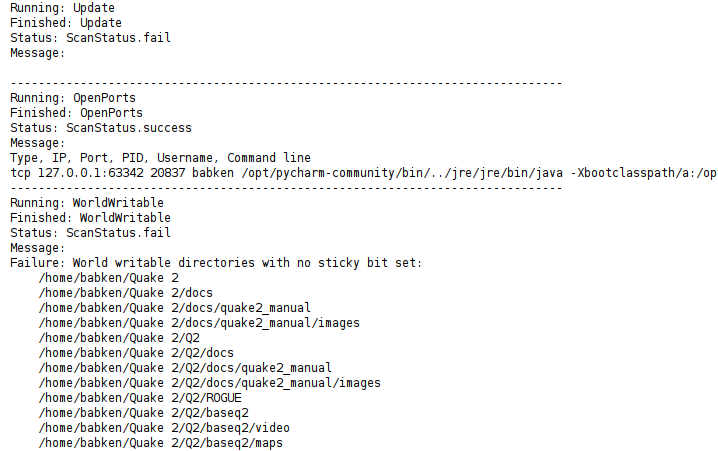
\includegraphics[width=1.0\textwidth]{result.png}
\end{figure}


\end{document}
